% use paper, or submit
% use 11 pt (preferred), 12 pt, or 10 pt only

\documentclass[letterpaper, paper,11pt]{./AAS}		% for final proceedings (20-page limit)

\usepackage{bm}
\usepackage{amsmath}
\usepackage{subfigure}
\usepackage[colorlinks=true, pdfstartview=FitV, linkcolor=black, citecolor= black, urlcolor= black]{hyperref}
\usepackage{xfrac}
\usepackage{booktabs}

\begin{document}

\subsection{$\Delta V$EGA Maneuver Implementation}
A $\Delta V$EGA orbit, also referred to as a leveraging orbit specifically of Earth, launches with the intent to gravity assist off the body for a higher post-flyby heliocentric energy\cite{Hollenbeck}.  Leveraging orbits are classified by their nominal resonance period multiple with respect to the flyby body's heliocentric orbit, and we will refer to this number as "$k$." For example, a leveraging orbit that has a period roughly 3 times as large as Earth's will have a $k=3$ which is represented as a 3:1 $\Delta V$EGA trajectory. The actual period of these orbits will vary either greater than or less than the nominal time due to flying by the body at a different Earth heliocentric true anomaly. Trajectories with a larger period are referred to as $k$:$1^{+} \Delta$VEGA and those with a shorter are $k$:$1^{-} \Delta$VEGA trajectories. To modify the flyby Earth true anomaly a maneuver at the aphelion (deep space maneuver) is executed.
\\\indent The deep space maneuver (DSM) and subsequent Earth launch characteristics are calculated before the tree generation in order to reduce the required number of computations within the search. We approximate the $\Delta$V requirements for both maneuvers, and their inclusion reduces the discontinuous trajectory endpoint velocities needed to patch Earth-Earth flyby sequences. Having the required aphelion $\Delta$V can also aid the optimization process initial guess. A lookup table sorted by the nominal resonance multiple ($k$) and encounter true anomalies ($\theta_{E}$) contains the resulting leveraging orbit properties and maneuver magnitudes. Due to being a rough approximation, the circular Earth orbit and coplanar trajectories assumptions are used. Finding the $\Delta V$EGA orbit parameters for a specific encounter true anomaly ($\theta_{E}$) and $k$ begins by assuming a nominal orbit period launch and its associated $V_\infty$. The state elements are computed at Earth and the resulting aphelion radius and velocity are found. Because the intercept true anomaly is fixed, its location and the time it takes to reach the point are known. Eq.~\eqref{eq:dteqn} is the difference in time from the DSM maneuver location to the Earth gravity assist (EGA) point where $T_E$ is the orbital period of Earth.
%
\begin{equation}
	\label{eq:dteqn}
	dt = kT_E \pm T_E(\theta_E/2\pi)
\end{equation}
%
%
\begin{figure}[htb]
	\centering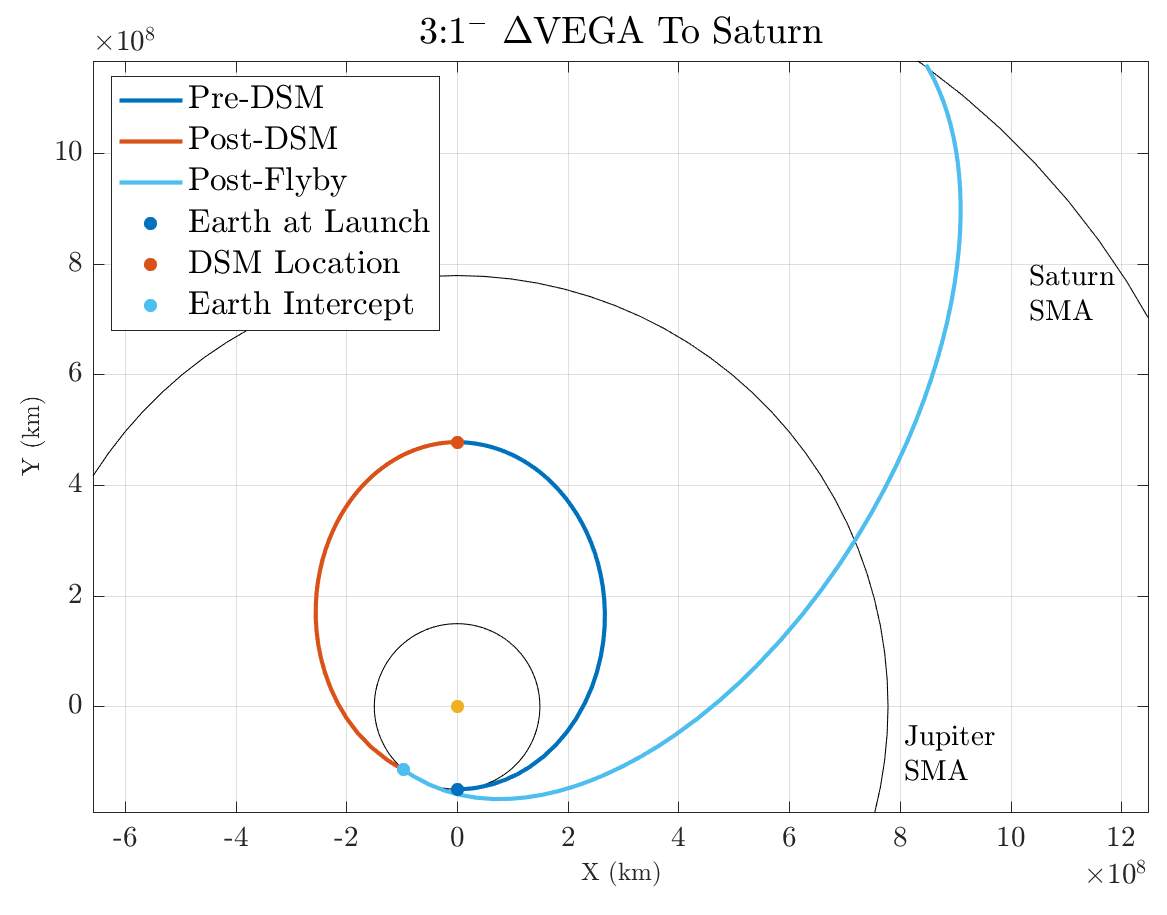
\includegraphics[width=3.6in]{./Figures/dsmmatlab}
	\caption{Example of a computed 3:$1^{-} \Delta$VEGA trajectory to Saturn's semi-major axis. The launch $V_\infty$ is 6.97 km/s and the required DSM $\Delta$V is 0.39 km/s. The EGA flyby altitude was constrained to 200 km, which yielded the highest post flyby energy.}
	\label{fig:dsmmatlab}
\end{figure}
%
\\A Lambert arc is computed between these points and the resulting initial velocity change is used to find the DSM vector. The final velocity vector is assumed to be the heliocentric velocity of the leveraging orbit at the EGA. The relative velocity, $\vec{V_\infty}$ is computed and a planar flyby of Earth can now be calculated from the tree search algorithm. Fig.~\ref{fig:dsmmatlab} illustrates an example leveraging orbit being calculated for $\theta_{E}$ = 40.$7^{\circ}$. An energy maximizing flyby and propagation to the new aphelion is added to the end of the $\Delta V$EGA orbit to show the resulting trajectory.
\\\indent From testing, we noticed that as $\mid\theta_E\mid$ increased, a normal component of the DSM $\Delta$V appeared and grew larger. To limit the $\Delta$V to only a tangential component, and in return to reduce the total $\Delta$V required, a minimizer can be employed. This optimization comes at the expense of a higher launch energy and a longer flight time for trajectories requiring large $\mid\theta_E\mid$. Differing trends from Sims et. al. analysis of $V_\infty$ leveraging\cite{sims1994} were only noticed in high total $\Delta$V cases for each $k$ leveraging orbit family. These solutions were discarded from the lookup table due to delivering lower aphelion radii post-flyby when compared to lower total $\Delta$V leveraging orbits of the same family. The case presented in Fig.~\ref{fig:dsmmatlab} is intended to matche that discussed by Sims et. al\cite{Sims1997} and has nearly identical results. The inclusion of deep space maneuvers, not specific to $\Delta V$EGAs, are not implemented in the current form of the tree search. However, because the algorithm patches the two conics forming the leveraging orbit using the Lambert's method, the possibility to extend DSM maneuvers for off-tangent $V_\infty$ departures and targeting for the flyby can be implemented. This inclusion adds another dimension to the lookup table but offers leveraging maneuvers between Earth and Venus.
\\\indent Now that the $\Delta V$EGA orbit properties are known, the lookup table solution can be extended to the actual solar system model in the tree search. The table values are represented in a relative frame with respect to Earth's state vector at the launch epoch. A subsequent transformation of the departure velocity and pre-EGA incoming $\vec{V_\infty}$ can be done in order to find their specific components corresponding to an Earth epoch in the Ecliptic J2000 frame. From the initial node in the tree, a set of Earth leveraging time-of-flight nodes are created corresponding to their respective $k$ and $\theta_E$ parameters. The number of these leveraging nodes included in the initial flight time layer of the tree is directly related to the angular spacing of $\theta_E$. As the resolution becomes finer, by increasing the $\textit{detail}$ input to the search, the estimated $\Delta$V becomes more accurate. This, however, increases of the number of tree nodes created, and so for a rough idea of the trajectory search space, a coarse resolution is preferred. The discontinuous $\Delta$V post-EGA required to patch the incoming leg from the leveraging orbit and outgoing leg to the next planet node will determine if the leveraging node and its performance is effective for the transfer. Using this method, a distinction between the $\Delta V$EGA trajectory families to different outer planets can be observed.


% Force the text below to next page
\phantom{p. 1}
\clearpage



\subsection{Case 3: Triton $\Delta V$EGA Opportunity Search}
The tree search algorithm can now be extended to an exploratory context to find possible trajectories for future concepts. With the interest in icy moon exploration in the solar system, a sequence to Neptune, and in return Triton, is explored\cite{Hubbard2010}. An arbitrary launch period was selected for this evaluation. The search is limited to trajectories with the inclusion of a $\Delta V$EGAs to evaluate its integration and performance. The number of iterations was set at 10,000 as this is seen to have a good compromise between calculation time and the number of search results. For a sequence to Neptune, it is desired to have a higher incoming relative velocity at Jupiter in order to have the appropriate outgoing energy to reach Neptune. With this in mind, the intent of the search was to find $\Delta V$EGA trajectories that deliver a high post EGA semi-major axis. The $\textit{detail}$ option is set to 16 which creates 8 $k$:1$^{-}$ and 8 $k$:1$^{+}$ nodes for each $k$ family. This spread is seen to balance the computation time (because of the number of nodes created) and the accuracy of the  DMS $\Delta$V. The C3 is set to emphasize the use of 2:1 $\Delta V$EGAs and the 3 and 4 $k$ leveraging families  would include the additional required velocity in the unoptimized $\Delta$V. The angular dispersion was set to 22 degrees yielding a fairly dense search space solution set. The results of the input search space are summarized in Table~\ref{tab:tritonInputs}:
%
%
\begin{table}[h]
    \begin{center}
        \caption{Inputs for $\Delta V$EGA Trajectories to Neptune via Jupiter}
        \label{tab:tritonInputs}
        \begin{tabular}{l|c}
					\toprule
            \textbf{Input Name} & \textbf{Input Value}\\
            \hline
            Arrival Planet & Neptune \\
            Launch Window \quad \quad & Jan 01, 2029 --- Jul 01, 2029 \\
            Iterations & 10,000 \\
            $\Delta V$ Budget & 4.5 $\sfrac{km}{s}$ \\
            Max C3 & 35 $\sfrac{km^2}{s^2}$ \\
            Detail ($d$) & 16 \\
						\bottomrule
        \end{tabular}
    \end{center}
\end{table}
%
%
\\\indent The search completed in 700 seconds and resulted in 1714 sequences from the 178,545 nodes created. As expected, most solutions used the 2:1 or 3:1 leveraging maneuvers, and a few 4:1 and direct EJN sequences were found with large unoptimized $\Delta$Vs.
$\textbf{Need to finish discussion on the search results.}$
\\\indent Fig.~\ref{fig:maltotriton} shows two optimized trajectories resulting from the search. The left plot is an example of a 2:1$^{+}$ $\Delta V$EGA which requires a launch $V_\infty$ magnitude of 5.39 $km/s$.
\\$\textbf{Need to finish discussion on MALTO plot below.}$
%
%
\begin{figure}[ht]
		\centering
		\begin{minipage}{0.50\textwidth}
				\centering
				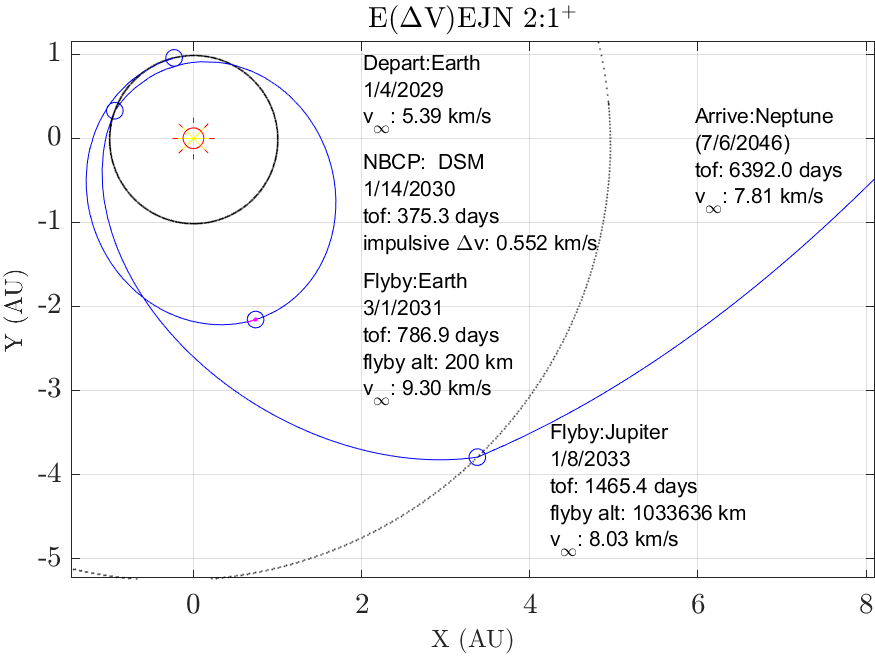
\includegraphics[width=1.0\textwidth]{./Figures/eejn21plus}
    \end{minipage}\hfill
		\begin{minipage}{0.50\textwidth}
				\centering
				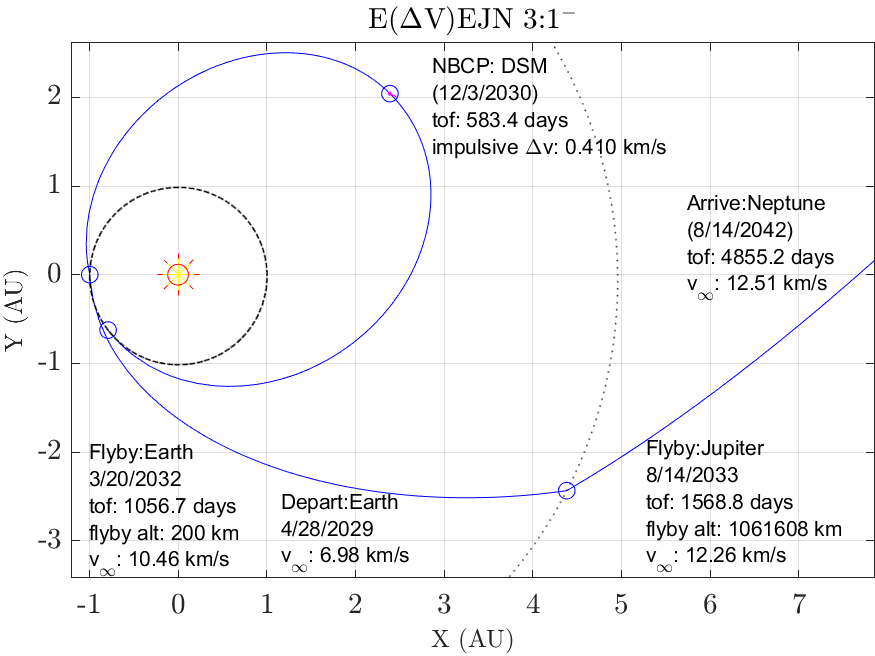
\includegraphics[width=1.0\textwidth]{./Figures/eejn31minus}
		\end{minipage}
		\caption{Optimized trajectory examples from the search. The left plot is an example of a 2:1$^{+}$ and the right is a 3:1$^{-}$. The 2:1$^{+}$ is able to reach Neptune with a much lower $V_\infty$ due to a slower relative velocity into Jupiter when compared to the 3:1$^{-}$ sequence.}
		\label{fig:maltotriton}
\end{figure}
%
%
\\$\textbf{Need to add discussion on leveraging performance}$
The deep space maneuver magnitude and direction vary from the search results due to various factors. The optimization process takes into account the change in declination for the outgoing flyby and so depending on the transfer, an additional Z-component of velocity is added by the optimizer to target the appropriate Earth flyby B-Plane angle. Another source of discrepancy is in the maneuver location. In the lookup table, the assumption is that the deep space maneuver is conducted at the aphelion of the leveraging orbit. In practice, the maneuver can be shifted before of after by the optimizer. Table~\ref{tab:} summarizes a few optimized cases and their predicted DSM $\Delta$V versus the calculated value from the optimization process.


The search returns several cases of interest which have been optimized and shown in Fig.~\ref{fig:maltotriton1} and Fig.~\ref{fig:maltotriton2}. Sequences that utilize a 2:1$^{-}$ and 2:1$^{+}$ have the lowest launch energy, but also have fairly large deep space maneuvers. The
\\$\textbf{THIS PART IS NOT DONE YET}$


\phantom{p. 1}
\clearpage
\bibliographystyle{./AAS_publication}
\bibliography{./referencesDSMSsection}

\end{document}
